\chapter{Boundary Conditions}

see exercise 3.2

\section{Location}

\section{Subsoil}

\section{Reference levels}

\section{Bathymetry}

\section{Waves}
Wave heights and the return period of wave events are essential for determine the dimensions of a breakwater. Especially for estimating the size of the amour layer and hence the size of under-layer material, is the wave hight the dominant parameter. Furthermore the order of the run-up and over-topping magnitude is mainly dependent on the wave hight.
\subsection{Design storm}
The design storm with less than 20\% probability of failure of the breakwater within a lifetime of 100 years returns every 500 years.
The available 22 years of (modelled) wave data\footnote{ARGOSS XX} close to the site is analysed in a Peak over Threshold analysis using a threshold of $H_s=1.5m$, a storm duration of nine hours and a Weibull distribution to extrapolate the data.
This yields a significant wave height of $H_{ss}=7.91m$ for a 500 year storm, which is chosen to be the deep water design wave height: $H_{ss,d}=7.91m$.

According to the distribution of the wave hight over peak wave periods from the wave model of Argoss %(appendix \ref{Distribution_pperiod}) 
the peak period was chosen to be 11 seconds.
The Distribution of the wind and the wind speed at 10 m hight was created through the Argoss data set too and shows velocities up to 20 m/s with varying directions
%\ref{Windrose}
. The main  directions are NW, N, NE, SSE and S but for the model just NW and S winds are considered with 20 m/s because of the influence at the breakwater as a worst case scenario.

\subsection{Near-shore Wave model}
SwanOne was used to estimate the wave development at near-shore. The Input parameters are in this case:
\begin{itemize}
\item the generated two dimensional bathymetry
\item the wave hight
\item peak period
\item wind velocity
\item angle of incidence 	
\end{itemize}
In the Swan model we included the set up due to wave action but we neglected additional wind, because it is included in the offshore wave data we gained and currents were neglected due to the location in the Mediterranean See with hardly any currents.
Bathymetry, wave hight, wind velocity and peak period were determined before, but now different angles of wave attack need to be considered.
For determine which angles are of interest for the occurrence of sea and swell waves the Argoss data are checked again 
%\ref{wavedata_angle}
. As a result from the analysis the dominant direction for waves to occur are NW and S, which matches with the geographical expectations. Due to the orientation of the breakwater at the coast the waves from NW will arrive with a very large angle close to 90$^\circ$ according to the breakwater why the wave energy attacking the breakwater is quite small. Because of the small fetch length just wave with relative low energy will arrive perpendicular to the breakwater. The biggest influence is expected to come from the south and thus the angle of the waves to attack the breakwater will be around 45$^\circ$ which is the value used for the modulation in SwanOne. The model was simulating with a grid size of around 5.55 m per cell and 10,000 time steps per simulation to get an accurate result.

The final Simulation is shown in figure %\ref{Hsig_Depth_Plot} 
and the actual value for the significant design wave hight from a one in 500 years storm at the near-shore in a depth of 12 meter is 5.614 m.
\begin{figure}[H]
\center
\fbox{
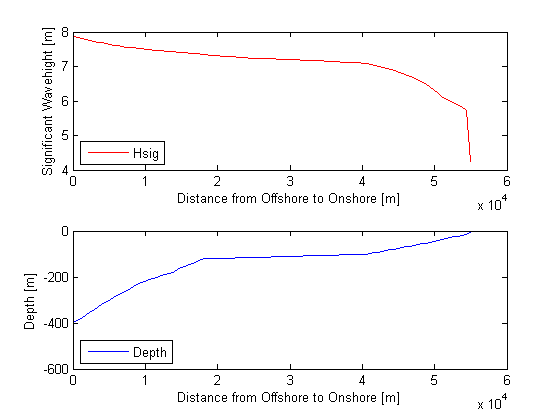
\includegraphics[width=\textwidth]{images/Hsig_Depth_Plot.png} 
}
\caption{Rose-diagram waves}
%\label{Hsig_Depth_Plot}
\end{figure}
